\section{Introduction}
I have spent the majority of my time this week participating in the Summer School on Human - Computer Interaction and trying to improve the Convolutional Neural Network last week.

\section{Summer School}
This is a 1-week summer school to introduce the Human-Computer interaction field by Mr. Le Khanh Duy. In this summer school there are presentations by speakers such as Prof. Morten Fjeld, Prof. Shengdong Zhao, Prof Kening Zhu and Prof. Tran Minh Triet

Here were some certificates that I receive during Summer School.

\begin{center}

\includegraphics[width=200pt]{week5-hci-certificate.jpg}
\end{center}

\section{Image Classification using CIFAR10}
\subsection{Convolutional Neural Network v2}
I tried modifying some configurations on model v1 to achieve higher accuracy. I changed from BatchNorm\cite{batchnorm} to DropOut. Here is my v2 architecture:
\begin{center}
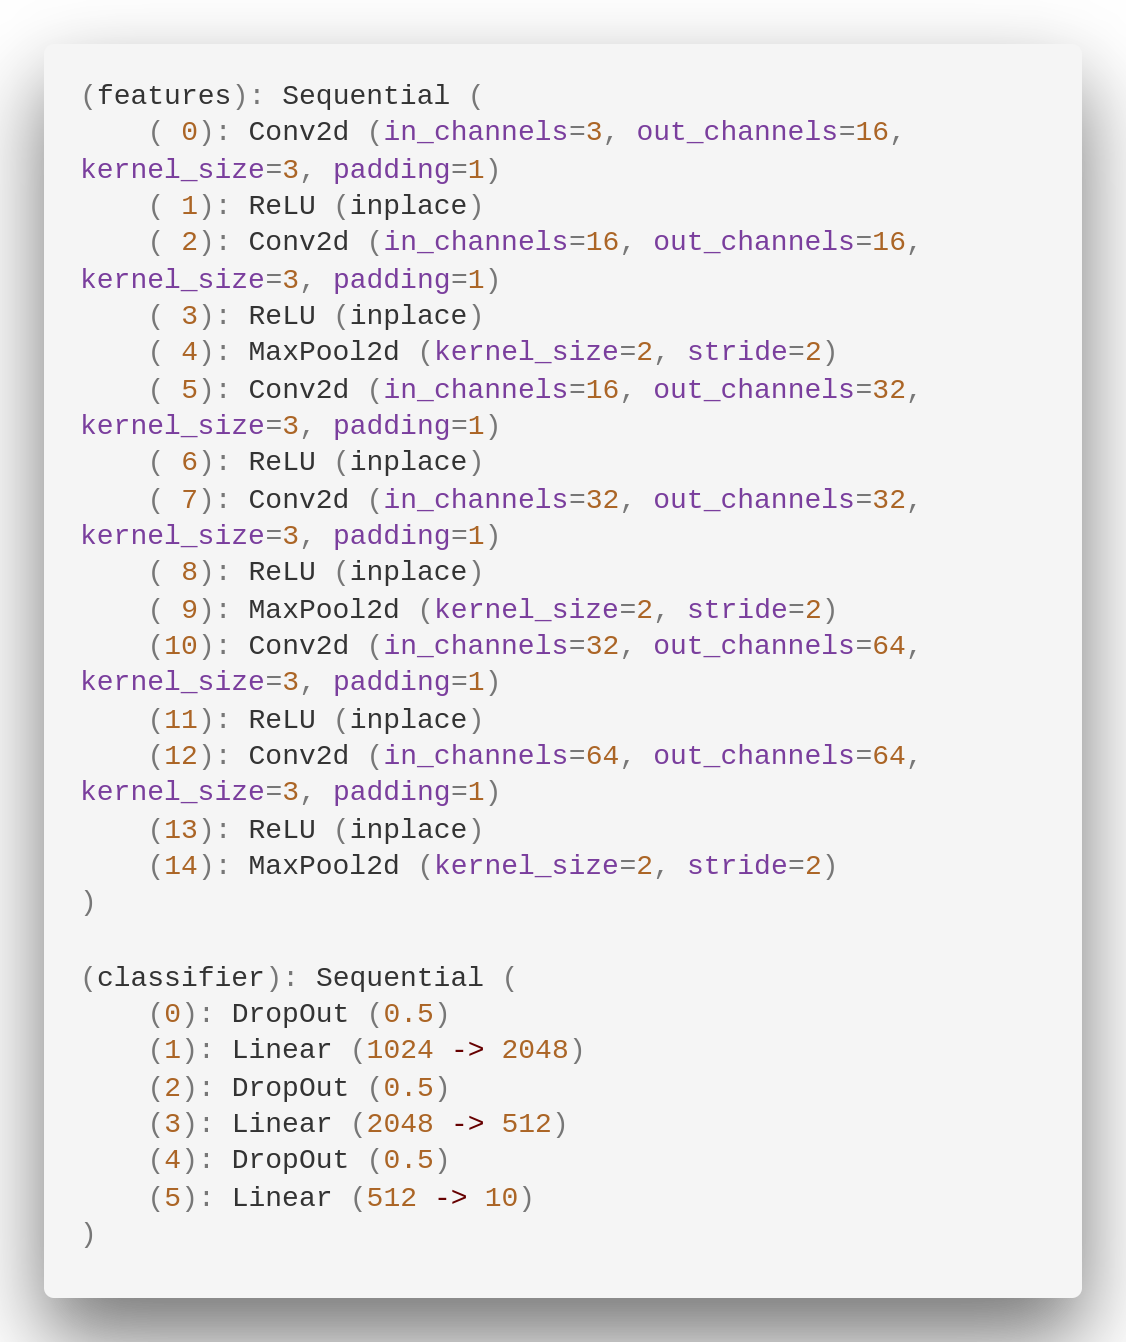
\includegraphics[width=\textwidth]{week5-model-architecture-v2.png}
\end{center}

I also increased the number of epochs to 300.

The training time increased from 18 mins to 55 mins, but I got the test error decreasing to 25.47\% (decrease 4.49\% compared to the v1 model).

\subsection{Convolutional Neural Network v3}
I continued modifying some configurations on model v2 and hoped for higher accuracy. I changed the learning rate, instead of using only one learning rate during training process, I tried 3 different learning rates which are:
\begin{itemize}
\item 1e-1 for epochs [0, 100)
\item 1e-2 for epochs [100, 200)
\item 1e-3 for epochs [200, 300]
\end{itemize}

The training time was not change, and I got the test error decreasing to 23.9\% (decrease 1.57\% compared to the v2 model).

And so far v3 model is the best one in term of the test error that I have.

\subsection{Source code}
All of my model architectures, detailed configurations, results and trained model could be found \href{https://github.com/tlvu2697/image-classification-cifar10}{on my GitHub}.